\documentclass{beamer} \usetheme{Madrid}
\usecolortheme{beaver}

\usepackage[utf8]{inputenc}
\usepackage{mdframed}
\usepackage{minted}
\usepackage{xcolor}

\newenvironment{question}[1][]{
	\ifstrempty{#1}{}
	{\mdfsetup{
			frametitle={
					\tikz[baseline=(current bounding box.east),outer sep=0pt]
					\node[anchor=east,rectangle,fill=gray!30]
					{#1};
				}
		}}
	\mdfsetup{
		innertopmargin=10pt,linecolor=gray!30,
		linewidth=2pt,topline=true,
		frametitleaboveskip=\dimexpr - \ht\strutbox\relax
	}
	\begin{mdframed}
		}{
	\end{mdframed}
}

\title{C++ Workshop}
\subtitle{Spring 2021}

\author[]{Jack Leightcap\inst{1}\inst{2}}

% this is pretty pretentious lmao
\institute[IEEE, Wireless Club]{
	\inst{1}IEEE -- \url{nuieeeofficers@gmail.com}
	\and
	\inst{2}Wireless Club -- \url{nuwirelessclub@gmail.com}
}

\date[Spring 2021]{March 15, 2021}

\begin{document}
\frame{\titlepage}

\begin{frame}
	\frametitle{Background, Workshop Structure}
	\begin{itemize}
		\item The C++ you see in classes is very different than the C++ you might see on co-op
		\item Compare both with 3 examples you might've seen in Embedded Design
		\item Some tools that can help with writing C++ programs
	\end{itemize}
	\vfill
	General notes:
	\begin{itemize}
		\item Ask questions at any time!
		\item Reach out to me on Slack with any lingering questions
	\end{itemize}
\end{frame}

\begin{frame}
	\frametitle{C++ versus C}
	\vfill
	\begin{table}[]
		\begin{tabular}{l|l}
			\multicolumn{1}{c|}{\textbf{C}} & \multicolumn{1}{c}{\textbf{C++}}   \\
			\hline
			\ldots well, C                  & old: ``C with classes''            \\
			                                & new: distinct language, roots in C \\
			control, specificity            & faster development                 \\
			``close to the machine''        & high-level
		\end{tabular}
	\end{table}
	\begin{center}
	\end{center}
	\vfill
	``There are only two kinds of languages: those that people [complain] about and those that nobody uses.'' -- Bjarne Stroustrup, \texttt{comp.lang.c++}\\[1em]
	``Within C++, there is a much smaller and cleaner language struggling to get out'' -- Bjarne Stroustrup, \underline{The Design and Evolutions of C++} [1994]
	\vfill
\end{frame}

\begin{frame}[fragile]
	\frametitle{Linked Lists: C with Classes Style}
	\begin{columns}
		\begin{column}{{0.4\textwidth}}
			\begin{minted}[fontsize=\footnotesize]{C++}
class node {
public:
  int val;
  node *next;
};

int main(void) {
  node *n1 = new node();
  node *n2 = new node();
  n1->val = 2;
  n1->next = n2;
  n2->val = 3;
  n2->next = NULL;
  return 0;
}
			\end{minted}
		\end{column}
		\begin{column}{{0.4\textwidth}}
			\begin{itemize}
				\item Replace a few things and this is a valid C program
				\item Fittingly with a memory leak
				\item Obvious here, not so much with more complexity
			\end{itemize}
		\end{column}
	\end{columns}
\end{frame}

\begin{frame}[fragile]
	\frametitle{Linked Lists: Modern-ish C++}
	\begin{columns}
		\begin{column}{{0.4\textwidth}}
			\begin{minted}[fontsize=\footnotesize]{C++}
#include <forward_list>

using std::forward_list;
int main(void) {
  forward_list<int> list;
  list.assign({2, 3});
  return 0;
}
			\end{minted}
		\end{column}
		\begin{column}{{0.4\textwidth}}
			\begin{itemize}
				\item Concise, less error-prone
				\item Don't need to worry about internals of a linked list, just the interface
				\item Want a doubly linked list? Just drop in \texttt{list} in place of \texttt{forward\_list}
			\end{itemize}
		\end{column}
	\end{columns}
\end{frame}

\begin{frame}[fragile]
	\frametitle{Memory: C with Classes Style, \texttt{new} and \texttt{delete}}
	\begin{columns}
		\begin{column}{{0.4\textwidth}}
			\begin{minted}[fontsize=\footnotesize]{C++}
void PointersSuck() {
  Song *pSong =
    new Song("Stacy's Mom",
	     "Fountains of Wayne");

  // use pSong...
  // don't lose track of it...

  // many lines, files away:
  delete pSong;
}
			\end{minted}
		\end{column}
		\begin{column}{{0.4\textwidth}}
			\begin{itemize}
				\item \emph{Explicit} memory management
				\item \texttt{new} pair \texttt{delete} \(\leftrightarrow\) \texttt{malloc} pair \texttt{free}
			\end{itemize}
		\end{column}
	\end{columns}
\end{frame}

\begin{frame}[fragile]
	\frametitle{Memory: Modern-ish C++, Smart Pointers}
	\begin{columns}
		\begin{column}{{0.4\textwidth}}
			\begin{minted}[fontsize=\footnotesize]{C++}
#include <memory>
using std::unique_ptr;
void SmartPointer() {
  unique_ptr<Song> pSong(
    new Song("Stacy's Mom",
	     "Fountains of Wayne")
  );

  // go crazy!

  // pSong is automatically deleted
}
			\end{minted}
		\end{column}
		\begin{column}{{0.4\textwidth}}
			\begin{itemize}
				\item \emph{Automatic} memory management
				\item The language figures out where to free memory
				\item Very simple form of \emph{Garbage Collection}
			\end{itemize}
		\end{column}
	\end{columns}
\end{frame}

\begin{frame}[fragile]
	\frametitle{Sorting: C with Classes Style}
	\begin{columns}
		\begin{column}{{0.4\textwidth}}
			\begin{minted}[fontsize=\footnotesize]{C++}
void ssort(int a[], int n) {
  int ii, jj, min_idx;
  for (ii=0; ii<n-1; ii++) {
    min_idx = i;
	for (jj=ii+1; jj<n; jj++)
	if ([jj]<a[min_idx]
	  min_idx = j;
	swap(&a[min_idx], &a[ii]);
  }
}
			\end{minted}
		\end{column}
		\begin{column}{{0.4\textwidth}}
			\begin{itemize}
				\item Implement a sorting algorithm I guess?
				\item Lots of control, can very carefully pick algorithm
			\end{itemize}
		\end{column}
	\end{columns}
\end{frame}

\begin{frame}[fragile]
	\frametitle{Sorting: Modern-ish C++}
	\begin{columns}
		\begin{column}{{0.4\textwidth}}
			\begin{minted}[fontsize=\footnotesize]{C++}
#include <algorithm>

// STANDARD SORTING
std::sort(a.begin(), a.end());

// SORTING IN REVERSE ORDER
std::sort(a.begin(), a.end(),
  [](auto a1, auto a2) {
     return (a1 > a2)
  }
);

// SORTING ABSOLUTE VALUE
using std::abs;
std::sort(a.begin(), a.end(),
  [](auto a1, auto a2) {
    return (abs(a1) < abs(a2));
  }
);
			\end{minted}
		\end{column}
		\begin{column}{{0.4\textwidth}}
			\begin{itemize}
				\item Less control over the actual algorithm used
				\item But super flexible!
				\item Trust experts' implementation
			\end{itemize}
		\end{column}
	\end{columns}
\end{frame}

\begin{frame}
	\frametitle{Tools: Linters (\texttt{clang-check})}
	\begin{itemize}
		\item Looks at your program (doesn't run it), and flags potential issues
		\item Syntact issues: forgot a semicolon, etc.
		\item Symantic issues: unfreed memory, types of arguments, etc.
	\end{itemize}
\end{frame}

\begin{frame}
	\frametitle{Lint: Syntax}
	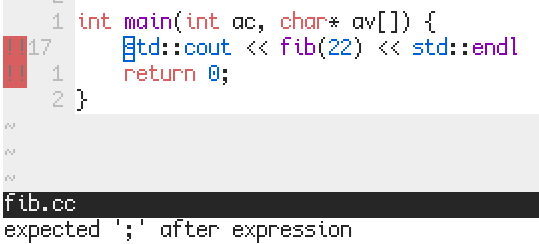
\includegraphics[width=\textwidth]{lint_syntax.png}
\end{frame}

\begin{frame}
	\frametitle{Lint: Symantic}
	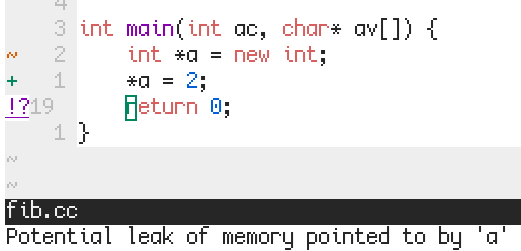
\includegraphics[width=\textwidth]{lint_symantic.png}
\end{frame}

\begin{frame}[fragile]
	\frametitle{Tools: Formatter (\texttt{clang-format})}
	\begin{itemize}
		\item Re-formats your program for consistency
		\item Helpful to agree on conventions when working with a team
	\end{itemize}
\end{frame}

\begin{frame}[fragile]
	\frametitle{Formatter: Example}
	\begin{columns}
		\begin{column}{{0.4\textwidth}}
			\begin{figure}[H]
				\begin{minted}[fontsize=\footnotesize]{C++}
int main()
{
  int ii=0;
  for(ii=0; ii<10; ii++)
  {
  if(ii%2==1)
    std::cout <<
	ii;
   	}
}
				\end{minted}
				\caption{Inconsistent formatting}
			\end{figure}
		\end{column}
		\begin{column}{{0.4\textwidth}}
			\begin{figure}[H]
				\begin{minted}[fontsize=\footnotesize]{C++}
int main() {
  int ii = 0;
  for (ii = 0; ii < 10; ii++) {
    if (ii % 2 == 1) {
      std::cout << ii;
    }
  }
}
			\end{minted}
				\caption{Automatically consistent}
			\end{figure}
		\end{column}
	\end{columns}
\end{frame}

\begin{frame}[fragile]
	\frametitle{Tools: Building}
	Compiler choices:
	\begin{itemize}
		\item Which compiler, \texttt{g++}, \texttt{clang++}, etc.
		\item Warnings: \texttt{-Wall}, \texttt{-Wextra}, \texttt{-Werror}, \texttt{-pedantic}, \texttt{-Wno-*}, etc.
		\item Optimization: \texttt{-pipe}, \texttt{-DNDEBUG}, \texttt{-O2}, \texttt{-Os}, etc.
		\item Standards: \texttt{-std=c++20}
		\item Debugging: \texttt{-ggdb}
	\end{itemize}
	Example compilation,
			\begin{minted}[fontsize=\footnotesize]{bash}
# All warnings, with debugging information
$ clang++ -Wall -Wextra -Werror -pedantic -ggdb file.cpp
			\end{minted}
\end{frame}

\end{document}
